\documentclass[conference]{IEEEtran}
\IEEEoverridecommandlockouts
% The preceding line is only needed to identify funding in the first footnote. If that is unneeded, please comment it out.
\usepackage{cite}
\usepackage{mathtools,amssymb,amsfonts,amsthm,bm}
\usepackage{algorithmic}
\usepackage{graphicx}
\usepackage{textcomp}
\usepackage{xcolor}
% Bibliography Package
	\usepackage[numbers]{natbib}
% Custom Packages
	\usepackage{tikz}
% Custom Commands
	\newcommand{\rx}{\mathsf{x}}
	\newcommand{\ry}{\mathsf{y}}
	\newcommand{\rs}{\mathsf{s}}
	\newcommand{\rz}{\mathsf{z}}
	\newcommand{\ru}{\mathsf{u}}
	\newcommand{\rsh}{\hat{\mathsf{s}}}
	\newcommand{\rzs}{(\mathsf{z}_t)_{t\in\NN}}
	\newcommand{\rss}{(\mathsf{s}_t)_{t\in\NN}}
	\newcommand{\rus}{(\mathsf{u}_t)_{t\in\NN}}
	\newcommand{\rxs}{(\mathsf{x}_t)_{t\in\NN}} 
	\newcommand{\rys}{(\mathsf{y}_t)_{t\in\NN}} 
	\newcommand{\rshs}{(\hat{\mathsf{s}}_t)_{t\in\NN}}
	\def\E{{\mathcal E}}
	\def\D{{\mathcal D}}
	\def\X{{\mathcal X}}
	\def\Y{{\mathcal Y}}
	\def\G{{\mathcal G}}
	\def\V{{\mathcal V}}
	\def\F{{\mathcal F}}
	\def\J{{\mathcal J}}
	\def\W{{\mathcal W}}
	\def\S{{\mathcal S}}
	\def\U{{\mathcal U}}
	\def\NN{{\mathbb N}}
	\def\QQ{{\mathbb Q}}
	\def\RR{{\mathbb R}}
	\def\ZZ{{\mathbb Z}}
	\def\FF{{\mathbb F}}
	\def\CC{{\mathbb C}}
	\def\mM{\bm{\mathrm{M}}}
	\def\mA{\bm{\mathrm{A}}}
	\def\mC{\bm{\mathrm{C}}}
	\def\mB{\bm{\mathrm{B}}}
	\newcommand{\QE}{\mathcal{Q}_{\mathrm{E}}}
	\newcommand{\QD}{\mathcal{Q}_{\mathrm{D}}}
	\newcommand{\oQE}{\overline{\mathcal{Q}}_{\mathrm{E}}}
	\newcommand{\oQD}{\overline{\mathcal{Q}}_{\mathrm{D}}}
	\newcommand{\BSS}{\mathrm{BSS}}
	\DeclareMathOperator{\Span}{Span}
	\newcommand{\rdummy}{{\color{red}[REF]}}
	\newcommand{\sdummy}{{\color{red}[SOURCE]}}
	\newcommand{\col}{\color{black}}
	\newcommand{\colol}{\color{orange}}
	%\newcommand{\tbr}[1]{{\color{gray}[#1]}}
	\newcommand{\tbr}[1]{}
	\newcommand{\noteholger}[1]{{\color{red}#1}}
% Custom Environments
	\newtheorem{Theorem}{Theorem}
	\newtheorem{Definition}[Theorem]{Definition}
	\newtheorem{Lemma}[Theorem]{Lemma}
	\newtheorem{Corollary}[Theorem]{Corollary}
	\newtheorem{Remark}[Theorem]{Remark}
%	%	%	%	%	
\def\BibTeX{{\rm B\kern-.05em{\sc i\kern-.025em b}\kern-.08em
    T\kern-.1667em\lower.7ex\hbox{E}\kern-.125emX}}
\begin{document}
%
	\title{Deciding the Problem of Remote State Estimation via Noisy Communication Channels on Real Number Processing Hardware
		\thanks{H.~Boche was supported by the German Research Foundation (DFG) within
				the Gottfried Wilhelm Leibniz Prize under Grant BO 1734/20-1, within
				Germany’s Excellence Strategy EXC-2111—390814868 and EXC-2092 CASA -
				390781972
				and by the German Federal Ministry of Education and Research (BMBF)
				within the national initiative for “Post Shannon Communication (NewCom)”
				with the
				project “Basics, simulation and demonstration for new communication
				models” under Grant 16KIS1003K.
				C.~Deppe was supported by the BMBF within NewCom with the project
				“Coding theory and coding methods for new communication models” under
				Grant 16KIS1005, by the German Research Foundation (DFG)
				with the Project "Post-Shannon theory and implementation" under Grant DE
				1915/2-1 and by the German Federal Ministry of Education and Research
				(BMBF) within the project "6G-life" under Grant 16KISK002.}
	}
	\author{\IEEEauthorblockN{Holger Boche}
	\IEEEauthorblockA{\textit{Institute for}\\ 
	\textit{Theoretical Information Technology,}\\
	\textit{Technical University of Munich}\\
	Munich, Germany\\
	boche@tum.de\\
	ORCID: 0000-0002-8375-8946}
	\and
	\IEEEauthorblockN{Yannik Böck}
	\IEEEauthorblockA{\textit{Institute for}\\ 
	\textit{Theoretical Information Technology,}\\
	\textit{Technical University of Munich}\\
	Munich, Germany \\
	yannik.boeck@tum.de\\
	ORCID: 0000-0001-7640-6988}
	\and
	\IEEEauthorblockN{Christian Deppe}
	\IEEEauthorblockA{\textit{Institute for}\\
	\textit{Communications Engineering,}\\
	\textit{Technical University of Munich}\\
	Munich, Germany \\
	christian.deppe@tum.de\\
	ORCID: 0000-0002-2265-4887}
	}

\maketitle

\begin{abstract}
	We consider a descision problem associated to the task of estimating the state of a dynamic plant remotely via a noisy communication channel: 
	given the descriptions of some unstable LTI plant, some LTI sensor and some DMC, does there exist a pair of encoder and decoder that 
	allows for the remote tracking of the plant's state with bounded error? Questions of this kind are becoming increasingly important in communication technologies, 
	since future communication networks are expected to incorporate distributed control and decision making. Analytically, this problem has been shown to involve the eigenvalues of the matrix 
	characterizing the plant's dynamic behaviour as well as the zero-error capacity of the DMC. Starting from this result, we approach the problem from the view of theoretical computer science, 
	with an explicit treatment of the unerlying machine Model. In particular, we prove that for every pair of a finite channel input alphabet and a finite channel output alphabet, there exists
	a Blum-Shub-Smale algorithm that computes the zero-error capacity in dependence of the channel matrix. Based on this, we devise a Blum-Shub-Smale algorithm that solves the above 
	decision problem given the plant's and DMC's characteristics. Blum-Shub-Smale machines are a promising candidate for a universal model of real number processing hardware, comparable
	to the Turing machine in the digital domain. Recently, we observe an increased interest in research and development towards real number and/or analog computing hardware, usually
	referred to by the term ``neuromorphic computing''. Since the requirements regarding hardware integrity and trustworthiness imposed on future communication networks has been shown
	to reach the fundamental limits of digital hardware, Blum-Shub-Smale machines merit an investigation from the theoretical point of view, even if they cannot be implemented as of today.  
\end{abstract}

\begin{IEEEkeywords}
	Computability, Blum-Shub-Smale Machines, Remote State Estimation, Noisy Channels, Zero-Error Coding 
\end{IEEEkeywords}

%\section{TO-DO}
	%\begin{itemize}
		%\item Check usage of \(j,J,k,K,l,L,\ldots\).
		%\item Check indents.
		%\item Sources and references.
		%\item Spellcheck.
		%\item Hypenation.
		%\item Emphasizement/Italic
		%\item \textbf{Revision.}
		%\item Conclusion (Why are results important?; Description on a BSS machine: BSS machines are able to handle exact descriptions, not ``representations of objects'',
				%as TMs do; Machine ethics; Big picture: other results on the topic; Different machine models lead to different results, making an explicit treatment of underlying
				%machine model necessary;).
		%\item ``Despite the fact..'': check styleguide.
		%\item ``BSS machines over \(\RR\) are regularly..'': check styleguide.
		%\item Almost sure stability.
		%\item Reference exact assumptions on \((\mA,\mB,W,\E,\D)\) and \((\rz_t)_{t\in\NN}\), \(\rs_{0}\).
		%\item Lemma \label{lem:SolvabilityCondition}: independent of distributions.
		%\item Sans-Serif versus normal notation (random variables versus realizations).
		%\item tbr Command!
	%\end{itemize}

%\tbr{Generally, remote and/or distributed decision making is becoming increasingly important in view of future communication networks. The ideas behin well known slogans like``Industry 4.0'', 
	%``Autonomous Driving'', ``Internet of Things'' and the ``Metaverse'' are examples for the currentd trend in communications to shift the focus away from pure data transmission 
	%towards interconnected information processing and control of agents that perform real world actions. Since technologies of this kind are potentially affecting human lives, 
	%strict rules for technology assessment are necessary. {\color{red} Der Übergang passt noch nicht...} For the upcoming 5G and 6G mobile communication standards,
	%explicite requirements regarding hardware trustworthiness and integrity are stated, some of which have been shown to exceed the limitations of today's digital hardware. 
	%At the same time, we can observe a recent paradigm shift in research and development towards analog signal processing and computing hardware, summarized under the slogan ``neuromorphic computing''. 
	%While the theoretical capabilities of digital hardware are precisely captured by the abstract model of Turing machines, a comparable universal model for analog computing has not been widely accepted. 
	%A promising candidate for the latter is the \emph{Blum-Shub-Smale} machine, a generalization of the Turing machine that can process exact real numbers. BSS machines have been shown to be more powerful
	%than Turing machines in general, with many specific instances of practical relevance. In particular, there are several scenarios in communication where BSS machines are more powerful than Turing machines.
	%Hence, BSS machines merit an investigation from a theoretical point of, even if they cannot be practically implementend as of today.}
	%\tbr{Given the rise of digital technology in control and decision making, questions of this kind become increasingly important, especially with regards to technology assessment and machine ethics.}

\section{Introduction}	\label{sec:Introduction}
	\IEEEPARstart{R}{emote} state estimation via noisy communication channels is a prominent problem in control theory 
	\cite{BL00, EM01, HOV02, IF02, HT05, HF02, L03, MS04, MS05, MS05a, MS05b, PS01, S06, SP03, TM04, TM04b, WB99}. 
	The problem involves both conotrol and communications. In praticular, as we will see in the following, the communications part is essential.  
	Informally, the corresponding dynamic system can be described as follows. The state of an unstable, linear, time-invariant plant is observed by a local sensor. 
	Subsequently, the sensor data is feed into an encoder that prepares the data for transmission trough a discrete, memoryless channel \emph{(DMC)}. 
	Based on the sequence of channel outputs, the remote decoder/estimator tries to estimate the current state of the plant. The setup is schematically depicted in Figure \ref{fig:Schematics}.
	\begin{figure}\linespread{1}
		\centering
		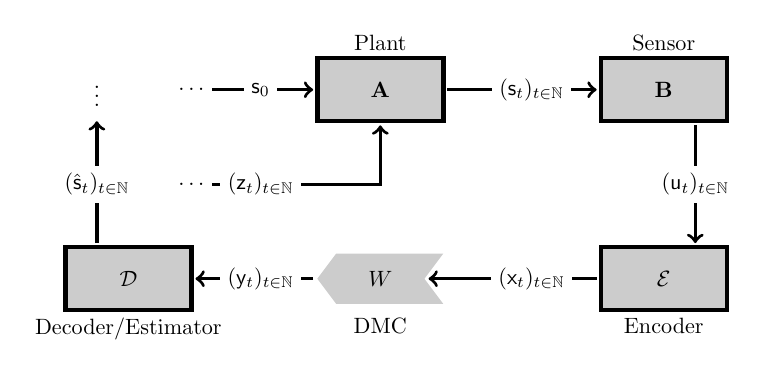
\begin{tikzpicture}[scale = 0.8, every node/.style={scale=0.8}]
			%   %   %   %   %   %   %   %   %   %   %
			%   Initial state
				\draw[very thick, ->, shorten >=1.5pt] (-4,1.5) -- (-2,1.5); 
				\draw (-2.9,1.5)  node[fill = white, anchor=center, align=center]
				{\(\rs_0\)};
				\draw (-4,1.5)  node[fill = white, anchor=center, align=center]
				{\(\dots\)};
			%   %   %   %   %   %   %   %   %   %   %
			%   Plant disturbance
				\draw[very thick, ->, shorten >=1.5pt] (-4,0) -- (-1,0) -- (-1,1); 
				\draw (-2.9,0)  node[fill = white, anchor=center, align=center]
				{\(\rzs\)};
				\draw (-4,0)  node[fill = white, anchor=center, align=center]
				{\(\dots\)};
			%   %   %   %   %   %   %   %   %   %   %
			%   Plant
				\draw[ultra thick, fill=black!20] (-2,2) rectangle (0,1);
				\draw (-1,1.5)  node[anchor=center] {\(\mA\)};
				\draw (-1,2)  node[anchor=south] {Plant};
			%   %   %   %   %   %   %   %   %   %   %
			%   Plant -> Sensor
				\draw[very thick, ->, shorten >=1.5pt, shorten <=1.5pt] (0,1.5) -- (2.5,1.5); 
				\draw (1.4,1.5)  node[fill = white, anchor=center]
				{\(\rss\)};
			%   %   %   %   %   %   %   %   %   %   %
			%   Sensor
				\draw[ultra thick, fill=black!20] (4.5,2) rectangle (2.5,1);
				\draw (3.5,1.5)  node[anchor=center] {\(\mB\)};
				\draw (3.5,2)  node[anchor=south] {Sensor};
			%   %   %   %   %   %   %   %   %   %   %
			%   Sensor -> Encoder
				\draw[very thick, <-, shorten >=1.5pt, shorten <=1.5pt] (4,-1) -- (4,1); 
				\draw (4,0)  node[fill = white, anchor=center, align=center]
				{\(\rus\)};
			%   %   %   %   %   %   %   %   %   %   %
			%   Encoder
				\draw[ultra thick, fill=black!20] (4.5,-2) rectangle (2.5,-1);
				\draw (3.5,-1.5)  node[anchor=center] {\(\E\)};
				\draw (3.5,-2)  node[anchor=north] {Encoder};
			%   %   %   %   %   %   %   %   %   %   %
			%   Encoder -> Channel
				\draw[very thick, ->, shorten >=1.5pt, shorten <=1.5pt] (2.5,-1.5) -- (-0.3,-1.5); 
				\draw (1.4,-1.5)  node[fill = white, anchor=center, align=center]
				{\(\rxs\)};
			%   %   %   %   %   %   %   %   %   %   %
			%   Channel
				\fill[fill = black!20] (-2,-1.5) -- (-1.7, -1.1) -- (0,-1.1) -- (-0.3,-1.5) -- (0,-1.9) -- (-1.7,-1.9);
				\draw (-1,-1.5)  node[anchor=center] {\(W\)};
				\draw (-1,-2)  node[anchor=north] {DMC};
			%   %   %   %   %   %   %   %   %   %   %
			%   Channel -> Decoder
				\draw[very thick, ->, shorten >=1.5pt, shorten <=1.5pt] (-2,-1.5) -- (-4,-1.5); 
				\draw (-2.9,-1.5)  node[fill = white, anchor=center, align=center]
				{\(\rys\)};
			%   %   %   %   %   %   %   %   %   %   %
			%   Decoder
				\draw[ultra thick, fill=black!20] (-6,-2) rectangle (-4,-1);
				\draw (-5,-1.5)  node[anchor=center] {\(\D\)};
				\draw (-5,-2)  node[anchor=north] {Decoder/Estimator};
			%   %   %   %   %   %   %   %   %   %   %
			%   State estimate
				\draw[very thick, ->, shorten <=1.5pt] (-5.5,-1) -- (-5.5,1);
				\draw (-5.5,0)  node[fill = white, anchor=center, align=center]
				{\(\rshs\)};
				\draw (-5.5,1.5)  node[fill = white, anchor=center, align=center]
				{\(\vdots\)};
		\end{tikzpicture}
		\caption{Schematics of the remote state estimation setup considered throughout this article. The setup is identical to the one introduced in \cite{BoBoDe21}\tbr{{\color{red}\(\leftarrow\) Change to TAC!~}}.}
		\label{fig:Schematics}
	\end{figure}
	The key applications of this problem range from robotics over autonomous driving to general remote controlled systems \cite{FeBo21}. However, there exist fundamental 
	limits to the capabilites of autonomous systems and computer aided design tools, as has been shown in several instances \cite{BoBoDe21}\tbr{{\color{red}\(\leftarrow\) Check this source!~}}. These fundamental limits essentially
	depend on the hardware in use. For digital hardware, the Turing machine determines the fundamental limits. In recent times, there has been an increasing interest in analog information processing.
	Here Blum-Shub-Smale machines are a good candidate for a universal computation model.
	
	In essence, the remote state estimation problem consists of designing a pair of encoder and decoder which allows for the estimation of the plant's state in a sufficient manner.
	Generally, this is known as the co-design of control and communication. In this context, the problem of remote state estimation via noisy channels is particularly interesting,
	since it is an example for a scenario where practically relevant control-performance criteria have an essential impact on the required communcations performance.
	As was shown in \cite{MS07}, the strong objective of almost sure observability requires the zero-error capacity of the DMC, while a weakened form of the observability criterion can be achieved
	by the classical Shannon capacity of the DMC.
	According to this, it is necessary to decide, based on the specifications of the plant and the DMC, whether an appropriate pair of encoder and decoder can exist in the first place. 
	Nowadays, this decision is often made by automated design tools or autonomous control units, e.g., in automated driving, either in an explicit or implicit way. In recent times, 
	\emph{digital twins} emerged as a further technique for handling design problems of this kind in practical applications. The approach is based on creating a full virtual copy of 
	the system on a digital computer, which is then employed for optimization, control tasks and decision-making. 

	From an analytic point of view, remote state estimation involves the disciplines of control and information theory. As indicated above, it is an explicit example of a so 
	called co-design problem. The practice of automated design and autonomous control adds another layer to the problem. In almost all cases, dynamic plants are analog, continuous  systems, 
	whereas the operation of digital computers is based on discrete algorithms. Hence, the question of whether appropriate computer-based decision-making with respect to analog 
	dynamic systems is actually possible, arises naturally. Thus, the question arises whether digital hardware is the proper hardware platform for decision making of this kind. It has been shown
	that digital hardware is insufficient in several cases. The Blum-Shub-Smale model is suitable to investigate whether analog information processing hardware, e.g., neuromorphic computing
	processors, is more suitable for this task.

	Problems of the latter kind are traditionally investigated in the field of theoretical computer science and have not gained much attention in applied engineering until now. 
	On the other hand, we can observe increasing requirements on electronic systems regarding safety, secrecy and, in lack of a different term, ethical behaviour \tbr{\sdummy}. 
	A prominent example is the related discussion surrounding autonomous driving, which is recently taking place in the community of machine ethics and technology assesment \tbr{\sdummy}. 
	In order to obtain a qualified evaluation of whether some digitally controlled technological system meets the abovementioned requirements, it is necessary to precisely understand 
	the fundametal boundaries of digital technology. This, in turn, requires an explicit treatment of those aspects of digital technology that involve theoretical computer science.

	In this series of articles (c.f. \cite{BoBoDe21X} for a full survey), we aim to approach the decision problem related to remote state estimation and stabilization from the perspective 
	of theoretical computer science. In \cite{BoBoDe21}\tbr{{\color{red}\(\leftarrow\) Change to TAC!~}}, we have considered the decision problem with regards to Turing machines. In this work, we instead discuss 
	\emph{Blum-Shub-Smale (BSS) machines} as the underlying machine model. Potentially, Blum-Shub-Smale machines yield a mathematical description of a universal analog computer.
	Regarding a practical implementation, however, there exist only individual examples of analog computation platforms, as, for example, from Intel, IBM and Samsung, until today. 
	
	Despite the fact that the capabilities real-world, digital computers are 
	entirely captured by Turing machines, BSS machines over \(\RR\) are regularly considered in numerics and computational complexity theory. 
	This practice is justified by the premise that the error emerging from representing real numbers by floating point approximations is neglectible in all practically relevant numerical problems. 
	Furthermore, assumptions on the underlying machine model are usually implicit in numerics. In contrast, we seek to explicitely treat the underlying machine model in our investigations.

	The outline of the remainder of this work is as follows. Sections \ref{sec:FormalEstimationSetup}, \ref{sec:PreliminariesBSS} and \ref{sec:PreliminariesZeroError} are dedicated to preliminaries. 
	In particular, we recapitulate the description of the remote state estimation setup in a formal manner and introduce the theory of Blum-Shub-Smale machines and zero-error coding.
	In Section \ref{sec:ComputingZeroErrorOnBSS}, we present a BSS algorithm which, for fixed channel input and output alphabets, computes the zero-error capacity as a function on 
	the set of channels. In \ref{sec:DecidingRemoteStateEstimationOnBSS}, we apply the results established in Section \ref{sec:ComputingZeroErrorOnBSS} to devise a BSS algorithm
	which, for a fixed characterization of the unstable plant, decides the solvability of the remote state estimation problem. 
	As already stated before the co-design of control and communication is of particular interest in this context, since the criterion for control performance, which is
	usually determined by the practical application, essentially determines the performance criterion for communication. Interestigly, the weakened form of the control performance criterion 
	is decidable on digital hardware, and thus requires not only a weaker communication performance, but also a weaker computation performance regardig decidability. 
	The paper closes with a subsumption of 
	our findings in Section \ref{sec:Conclusion}.
                                                                        
\section{Formal Description of the Remote State Estimation Setup}	\label{sec:FormalEstimationSetup}
	\noindent As indicated in Section \ref{sec:Introduction}, we consider the problem of remotely estimating the state of a dynamic plant via a noisy communication channel. 
	For a detailed treatment of the problem as such, we refer to \cite{MS07}. Schematically, the set-up is depicted in Figure \ref{fig:Schematics}. 
	The system is identical to the one introduced in \cite{BoBoDe21}\tbr{{\color{red}\(\leftarrow\) Change to TAC!~}}. In order to provide a self-contained work, we recapitulate 
	the description in the following.

	The remote state estimation setup is characterized by the quintuple \((\mA,\mB,W,\E,\D)\) and the random variables \((\rz_t)_{t\in\NN}\), and \(\rs_{0}\). 
	The latter model the sequence of probabilistic fluctuations disturbing the plant, as well as the plant's initial state, respectively. The plant's state sequence \((\rs_t)_{t\in\NN}\) 
	and the sequence of sensor data \((\ru_t)_{t\in\NN}\) obey the system of equations
	\begin{align*}	\rs_1    &= \mA \rs_0 + \rz_1, \\ 
					\rs_t    &= \mA \rs_{t-1} + \rz_t,\\ 
					\ru_t    &= \mB \rs_t,
	\end{align*}
	where \(\mA\in\RR^{n\times n}\) and \(\mB\in\RR^{n\times l}\) capture the plant's and sensor's characteristics. 

	The sequence of channel inputs \((\rx_t)_{t\in\NN}\) is a sequence
	of symbols from a finite alphabet \(\X\). It is calculated by the encoder based on available sensor data,
	\begin{align*}	\rx_t   &= \E \big(t, (\ru_{t'})_{t'=1}^{t}\big) \\
							&= \E\big(t, \ru_1,\ru_2,\ldots,\ru_t\big).
	\end{align*} 
	The sequence of channel outputs \((\ry_t)_{t\in\NN}\) is a sequence
	of symbols from a finite alphabet \(\Y\). It is component-wise related to the sequence \((\rx_t)_{t\in\NN}\) by a conditional probability mass function,
	\begin{align*}	W :~ \Y \times \X \rightarrow \RR_{\hspace{1pt}0}^+,~(y,x) \mapsto W(y|x).
	\end{align*}
	Last but not least, the decoder estimates the plant's state sequence based on the available channel outputs,
	\begin{align*}	\hat{\rs}_t  	&= \D \big(t, (\ry_{t'})_{t'=1}^{t}\big) \\ 
									&= \D\big(t,\ry_1,\ry_2,\ldots,\ry_t\big).
	\end{align*}

	The strong objective in remote state estimation requires almost sure observability. By a suitable choice of \(\E\) and \(\D\), the error between \((s(t))_{t\in\NN}\)
	and \((\hat{s}(t))_{t\in\NN}\) must be kept small along almost all possible trajectories \((\zeta(t))_{t\in\NN}\) and \((y(t))_{t\in\NN}\), i.e., with probability one.
	A corresponding mathematical framework, which most of the considerations within the present work will be based on, was established in \cite{MS07}.
	In particular, the authors derived a strong relation between the solvability of the remote state estimation problem and the zero-error capacity \(C_0(W)\) of the 
	communication channel, as introduced in \cite{Sh56}. If the channel is unsuitable for transmitting a sufficient amount of data with perfect reliability, i.e., zero 
	chance of a transmission error, the discrepancy between \(s(t)\) and \(\hat{s}(t)\) accumulates over time and grows arbitrarily large, even if \((\zeta(t))_{t\in\NN}\) 
	is bounded arbitrarily close to zero. In this case, an unstable dynamic plant cannot be observed remotely with a bounded error. 

\section{Preliminaries from the Theory of Blum-Shub-Smale Machines}	\label{sec:PreliminariesBSS}	    	
	\noindent Blum-Shub-Smale (BSS) machines formalize the notion of computability over a field \(\FF\). The latter is assume to be equipped 
	with a binary relation \(\diamond~{:}~\FF \times \FF \rightarrow \{\mathsf{T},\mathsf{F}\}\), which is either an equality, equivalence or strict total order. 
	
	Despite the so called Church-Turing thesis being widely accepted as true, which implies that the capabilities of real-world computers are exactly characterized 
	by the abstract Turing machine, BSS machines are often implicitely considered as the underlying machine model in numerics and complexity theory \tbr{\sdummy}. 
	A reason for this practice may lie in the ability of BSS machines to handle exact real numbers. Since most areas of applied mathematics involve continuous structures, 
	treating the content of a computer's memory as actual real numbers simplifys the description of algorithms to a great extent. For a detailed discussion on the Topic, we refer to \cite{Bl04}.

	In essence, BSS machines can be considered a generalization of Turing machines. They are equipped with a two-way infinite tape divided into cells, each of which holds an 
	element of \(\FF\cup\{\sqcup\}\). Here, "\(\sqcup\)" denotes the distinguished empty-space symbol. We assume that the tape is almost empty, i.e., all but finitely many cells 
	contain the symbol "\(\sqcup\)", at the beginning of the computation. A BSS machine interacts with its tape by means of a read-write head, which can, depending on tis current 
	position, access a fixed number of contiguous cells at a time. The algorithm executed by the BSS machine is characterized by its programm, a finite, directed, simple graph 
	\begin{align*}   \G_\BSS = ([M_\BSS]_{0}, \V_\BSS),~ \V_\BSS \subseteq [M_\BSS]_{0} \times [M_\BSS],
	\end{align*} 
	with five types of nodes: \emph{input nodes}, \emph{computation nodes}, \emph{branching nodes}, \emph{shifting nodes} and \emph{output nodes}, each of which specifies a class 
	of fundamental machine operations. For a given input, the programm flow corresponds to a directed walk in the programm graph
	\begin{align*}	\F := (e_t)_{t\in\{1,2,\ldots,T\}},~T\in\NN\cup \{\infty\},
	\end{align*}
	starting from the input node and (possibly) ending in some output node, or continuing infinitely. In each step, the operaton associated to the current node is executed, 
	affecting the content of the tape, the position of the read-write head and the programm flow accordingly. Furthermore, the values stored in the initially non-empty cells 
	of the tape are considered part of the algoritm, much like hard-coded constants in a real-world computer programm. 

	In order to prove that some problem is BSS-computable, on has, in principle, to provide the existence of a suitable programm graph and, possibly, a tape with predefined constants. 
	This can often be cumbersome, since it involves the exact specification of the movement of the read-write head. If the size of the \emph{memory} required to execute the programm, i.e., 
	the number of different cells accessed througout the programm execution, can be uniformly upper bounded by a number \(J_\BSS \in \NN\), we can get rid of the tape alltogether by 
	introducing \emph{register variables} and \emph{constants},
	\begin{align*}	\bm{r} :&= (r_j^t)_{j\in\{1,\ldots,J_{\mathrm{R}}\}, t\in\{1,\ldots,T\}},\\
					\bm{c} :&= (c_j)_{j\in\{J_{\mathrm{R}} + 1,\ldots,J_{\mathrm{C}}\}},
	\end{align*}
	with \(T\in\NN\cup\{\infty\}\) and \(J_{\mathrm{C}} \leq J_\BSS\). The programm graph then consists only of an input node, computation nodes, branching nodes and at least one output node.
	Furthermore, the corresponding classes of fundamental machine operations can be specified as follows:
	\begin{itemize}	\item[1)] \emph{Input nodes.} The unique input node \(\iota = e_1 = 0\) is associated to an 
						input operation \(g_\iota\). The input operation writes each component of a tuple 
						\begin{align*} 	\bm{a} = \big(a_1,a_2,\ldots a_{K({\bm{a}})}\big) \in \bigcup_{j=1}^{J_{\mathrm{R}}} \FF^{j}
						\end{align*}
						to the machine's internal registers \(\bm{r}\), according to the specificaton
						\begin{align*}	r^1_{j(k)} := a_k ,~ j(k)\in \{1,\ldots,J_{\mathrm{R}}\},~ k\in \{1,\ldots K(\bm{x})\}.   
						\end{align*}
						The remaining registers are initialized with the value\linebreak \(0 \in \FF\).
						There exists a unique next node \(\iota' \in [M_\BSS]\) to \(\iota\).
					\item[2)] \emph{Computation nodes.} The programm graph may contain a number of computation nodes \(\zeta \in \{1,2,\ldots M_{\mathrm{C}}\}\),    
						\linebreak \(M_{\mathrm{C}} \leq M_{\BSS}\), each of which is 
						is associated to a mapping 
						\begin{align*} 	g_\zeta : \FF^{J_{\mathrm{C}}}\rightarrow \FF^{J_{\mathrm{R}}}. 
						\end{align*} 
						which is either polynomial, rational or has previously been shown to be BSS computable. The latter accounts for the fact that in the general, 
						unbounded setting, the programm of some BSS machine can always be incorporated as a subroutine into the programm of another BSS machine.
						If \(e_t = \zeta\) for some \(t\in\{1,\ldots, T-1\}\), we have
						\begin{align*}  \bm{r}^{t+1} = g_{\zeta}(\bm{r}^t,\bm{c})~\text{with}~\bm{r}^t := (r_j^t)_{j\in\{1,\ldots,J_{\mathrm{R}}\}}.
						\end{align*}
						There exists a unique next node \(\zeta' \in \{1,2,\ldots M_{\mathrm{C}}\}\) to each computation node \(\zeta\).
					\item[3)] \emph{Branching nodes.}  A programm may contain a number of branching nodes \(\beta \in \{M_{\mathrm{C}} + 1, M_{\mathrm{C}} + 2,\ldots, M_\mathrm{B}\}\), 
						each of which leave the content of the internal registers unchanged. That is, if \(e_t = \beta\) for some \(t\in\{1,\ldots, T-1\}\), we have
						\(\bm{r}^{t+1} = \bm{r}^{t}\). There exist exactly two next nodes \(\beta'(\mathsf{T})\) and \(\beta'(\mathsf{F})\) to each branching node \(\beta\). If 
						\begin{align*}	\diamond\big(0, r^t_{j'(\beta)}\big) = \mathsf{T} 
						\end{align*}
						holds true for \(j'(\beta) \in \{1,\ldots, J_\mathrm{R}\}\), the programm flow branches to the node \(\beta'(\mathsf{T})\). Otherwise, it moves to \(\beta'(\mathsf{F})\). 
						That is, for \(\beta = e_t\), we have
						\begin{align*}   e_{t+1} =   \begin{cases}   \beta'(\mathsf{T})  &\text{if}~\diamond\big(0,r^t_{j'(\beta)}\big) = \mathsf{T},\\
																	\beta'(\mathsf{F})  &\text{otherwise}.
													\end{cases}    
						\end{align*}
					\item[4)] \emph{Output nodes.} Each programm contains at least one output node \(\sigma \in \{M_{\mathrm{B}} + 1, M_{\mathrm{B}} + 2,\ldots, M_\BSS\}\), 
						each of which is associated to an output mapping
						\begin{align*}	o_\sigma : \FF^{J_{\mathrm{C}}}\rightarrow \FF^{J_{\sigma}}.
						\end{align*}
						For some fixed subset \(\J_\sigma\) of \([J_\mathrm{C}]\) and \(e_t = e_T = \sigma\), \(T\in\NN\), the mapping outputs (by projection) the values of the 
						register variables \((r_j^T)_{j\in \J_\sigma \cap \{1,\ldots,J_\mathrm{R}\}}\) and constants \((c_j)_{j\in \J_\sigma \cap \{J_\mathrm{R}+1,\ldots,J_\mathrm{C}\}}\). 
						There exists no next node to \(\sigma\).
	\end{itemize}
	In our case, the field \(\FF\) will be the real numbers \(\RR\) with the usual strict total order "\(<\)". If \(\FF\) equals \(\ZZ_2\) (the set of boolean values with logical con- and disjunction 
	as field operations), the traditional theory of computation as formalized by Turing machines is recovered. For the remainder of this article, we will refer to BSS machines over \(\RR\) 
	simply as BSS machines, omitting the explicit mention of the field \(\FF\) being equal to the real numbers. 

\section{Preliminaries from the Theory of Zero-Error Coding}	\label{sec:PreliminariesZeroError}
	\noindent As indicated in Section \ref{sec:FormalEstimationSetup}, we consider finite alphabets \(\X\) and \(\Y\) as well as conditional probability mass functions on \(\Y\times\X\).
	In particular we define
	\begin{align*}	\W(\X,\Y)	:=	\Bigg\{ W: 	&~\X \times \Y \rightarrow\RR_{\hspace{1pt}0}^+, \\
												&~\forall x\in\X: \sum_{y\in\Y} W(x,y) = 1 \Bigg\}.
	\end{align*}
	Since \(W\in \W(\X,\Y)\) characterizes a conditional probability mass function, the values of \(W\) are denoted by \(W(y|x)\) rather than \(W(x,y)\).  
	The triple \((\X,\Y,W)\) is called a \emph{discrete, memoryless channel}. 

	The theory of zero-error coding, as introduced in \cite{Sh56}, is a sub-discipline of general channel coding. In essence, it considers the problem of finding the supremum 
	\(C_0(W)\) of all possible rates at which information can be transmitted trough a DMC \((\X,\Y,W)\) with perfect reliability. Here, ``perfect reliability'' refers
	to the ability of the decoder to correctly infer the transmitted message with probability one. Furthermore, the term ``rate'' denominates the asymptotic average of bits transmitted per channel use. 
	The number \(C_0(W)\) is commonly referred to as zero-error capacity of \(W\).

	Given a DMC \((\X,\Y,W)\), one of the results derived in \cite{Sh56} yields a characterization of \(C_0(W)\) in graph-theoretic terms.
	In fact, for each \(W\in \W(\X,\Y)\), there exists a finite, undirected, simple graph \(G(W)\), referred to as the \emph{confusability graph} of \(W\), which
	uniquely determines \(C_0(W)\).

	\begin{Theorem}	[\cite{Sh56}]\label{thm:ZE_Capacity}
					For a DMC \(W\in\W(\X,\Y)\), let \(G(W) = (\X, \V(W))\) be the finite, simple graph that satisfies
					\begin{align*}   \V(W) = \big\{\{x,x'\} : \exists y : W(y|x)W(y|x') > 0\big\}.
					\end{align*}
					Then, the zero-error capacity of \(W\) satisfies
					\begin{align*}   C_0(W)  	&=  \lim_{n\to\infty} \frac{1}{n} \log_2 \alpha\big(G^{\boxtimes n }(W)\big) \\
												&=  \sup_{n\in\NN} \frac{1}{n} \log_2 \alpha\big(G^{\boxtimes n }(W)\big),
					\end{align*}
					where \(G^{\boxtimes n }(W)\) denotes the \(n\)-fold \emph{strong graph product} of \(G(W)\) with itself and
					\(\alpha\big(G^{\boxtimes n }(W)\big)\) denotes the \emph{independence number} of \(\alpha\big(G^{\boxtimes n }(W)\big)\).
	\end{Theorem}
	
	In more than 60 years of research in information theory, the zero-error capacity has given rise to a number of famous problems, many of which remain
	unsolved to date \tbr{\sdummy}. In \cite{BD20Z}, it was shown that \(C_0(W)\) is not computable on a Turing machine as a function on computable channel descriptions \(W\).
	To the best of the author's knowledge, it remains an open problem whether \(C_0(W)\) is even a Turing computable number for all computable channel descriptions.
	In Section \ref{sec:ComputingZeroErrorOnBSS}, we describe a BSS-algorithm which, for fixed alphabets \(\X\) and \(\Y\), computes \(C_0(W)\) as a function on \(\W(\X,\Y)\), which
	essentially relies on the ability of BSS machines to handle exact real numbers.

\section{Computing the Zero-Error Capacity for Fixed Alphabets on Blum-Shub-Smale Machines}	\label{sec:ComputingZeroErrorOnBSS}
	\noindent In the following, we specify a BSS-Algorithm which, for fixed alphabets \(\X\) and \(\Y\), computes the zero-error capacity \(C_0(W)\) 
	upon being passed a channel description \(W \in \W_c(\X,\Y)\). 

	Essentially, the algorithm relies on the fact that a \emph{lookup table} containing all possible values of \(C_0(W)\) can be hard-coded into the programm. The lookup is performed in 
	terms of a perfect binary tree, where each branch corresponds to an evaluation of the predicate "\(W(y|x) > 0\)" for some letters \(x\in\X\) and \(y\in\Y\). Per definition, the latter 
	can be done algorithmically, as a fundamental operation on the BSS machine.

	\begin{Theorem}	\label{thm:ZeroErrorBSScomputable}
					Consider finite alphabets \(\X\) and \(\Y\). Then, there exists a BSS-Machine \(\BSS_{C_0}\)
					which, upon being passed a channel description \(W\in \W(\X,\Y)\), computes the mapping \(W \mapsto C_0(W)\).
	\end{Theorem}\begin{proof}
					Let \(j \mapsto \big(x(j), y(j)\big)\) be an enumeration of the set \(\X\times\Y\) and define
					\(J_\mathrm{R} := |\X\times \Y|\). Furthermore, consider the mappings
					\begin{align*}	\delta(W,j) :&=     \begin{cases}   1   &\text{if}~ 0 < W\big(y(j)|x(j)\big), \\
																		0   &\text{otherwise},
														\end{cases}\\
									\Delta(W)   :&=     1 + \sum_{j=1}^{J_\mathrm{R}} \delta(W,j)\cdot 2^{j-1} \in \big\{1,\ldots,2^{J_\mathrm{R}}\big\}.
					\end{align*} 
					We observe that, as a direct consequence of Theorem \ref{thm:ZE_Capacity}, the value of \(C_0(W)\) is 
					entirely determined by the set 
					\begin{align*}   \{(x,y) \in \X\times \Y : W(x|y) > 0\} \subseteq 2^{\X\times\Y}
					\end{align*} 
					and hence, the zero-error capacity of \(W\) depends exclusively on the number \(\Delta(W)\). Thus, we obtain the existence of a mapping
					\begin{align*}	C'_0 : \big\{1,\ldots,2^{J_\mathrm{R}}\big\} \rightarrow \RR_0^+,~ \Delta \mapsto C'_0(\Delta)        
					\end{align*}
					such that \(C'_0(\Delta(W)) = C_0(W)\) holds true for all \(W\in\W(\X,\Y)\). For \(J_\mathrm{C} := J_\mathrm{R} + 2^{J_\mathrm{R}}\), 
					hardcode the family of constants \(\bm{c}\) according to 
					\begin{align*}   c_j := C'_0(j - J_\mathrm{R})
					\end{align*}
					for all \(j\in \{J_\mathrm{R} + 1, \ldots, J_\mathrm{C}\}\) and specify the programm \(\G = ([M_\BSS],\V_\BSS)\) with
					\begin{align*}	M_\mathrm{C} := 0,~M_\mathrm{B} := 2^{J_\mathrm{R}} - 1,~ M_\BSS := ~M_\mathrm{B} + 2^{J_\mathrm{R}}
					\end{align*}
					in the following way:
					\begin{enumerate}	\item[\(\iota\)\hspace{1pt}:] Preallocate the machine's registers \(\bm{r} := \bm{r}^1\) according to
											\(r_j := r^1_j := W\big(y(j)|x(j)\big)\) and set \(\iota' := 1\). Since the programm does not contain any computation nodes,
											the content of the registers remains constant during the execution. We thus omit the superscript of the
											register variables in the following.
										\item[\(\beta\)\hspace{1pt}:] 
											For \(\beta \in \{1,\ldots, M_\mathrm{B}\}\), the pair of next nodes \(\big(\beta'(\mathsf{T}),\beta'(\mathsf{F})\big)\) satisfies
											\begin{align*} 	\beta'(\mathsf{T}) :    &=  2\beta + 1, \\
															\beta'(\mathsf{F}) :    &=  2\beta.
											\end{align*}
											Denote \(m\in\NN\) the smallest natural number such that \(\beta < 2^m\) is satisfied. If, for some \(t\in\{1,\ldots, T-1\}\), we have
											\(e_t = \beta\), then \(e_{t+1}\) satisfies
											\begin{align*}   e_{t+1} := \begin{cases}	\beta'(\mathsf{T}) &\text{if}~ 0 < r_m,\\
																						\beta'(\mathsf{F}) &\text{otherwise}.
																		\end{cases}
											\end{align*}
										\item[\(\sigma\)\hspace{1pt}:] For \(\sigma \in \{M_\mathrm{B} +1, M_\BSS\}\), set \(j(\sigma) := \sigma - M_\mathrm{B} + J_\mathrm{R}\) 
											and return \(c_{j(\sigma)}\).
					\end{enumerate}
					Then, the BSS machine \(\BSS_{C_0}\) characterized by the triple \((\bm{r}, \bm{c}, \G)\) computes the mapping \(W\mapsto C_0(W)\).
	\end{proof}

\section{Deciding the Solvability of the Remote State Estimation Problem on Blum-Shub-Smale Machines}	\label{sec:DecidingRemoteStateEstimationOnBSS}
	In this section, we will use Theorem \ref{thm:ZeroErrorBSScomputable} to derive a BSS algorithm which, given the description of an unstable, linear plant,
	decides the solvability of the remote state estimation problem as a function on \(\W(\X,\Y)\).
	
	Again, the algorithm essentially relies on the ability of BSS machines to handle exact real numbers 
	For \(\mA \in \RR^{n\times n}\), denote \(\bm{\lambda}(\mA) := (\lambda_1(A),\lambda_2(A),\ldots,\lambda_n(\mA))\) a family 
	consisting of all eigenvalues of \(\mA\), according to their algebraic multiplicity. Consequently, the family \(\bm{\lambda}(\mA)\)
	consists of exactly \(n\) components for all \(\mA\in \RR^{n\times n}\). We define
	\begin{align}	\eta(\mA):=\sum_{j:|\lambda_j(\mA)|\geq 1} \log_2|\lambda_j(\mA)|.
	\end{align}
	
	As indicated in the introduction, the zero-error capacity of the DMC \(W\) plays a central role in the solvability of the remote state estimation problem;
	in essence, given a characterization \((\mA,\mB,W,\E,\D)\) of a remote state estimation setup, it is almost entirely determined by the pair \((\mu(\mA),C_0(W))\).
	
	\begin{Lemma} 	[\cite{MS07}]\label{lem:SolvabilityCondition} Let \(\X,\Y\) be finite alphabets, \(W\in \W(\X,\Y)\) a DMC and \((\mA,\mB) \in \RR^{n\times n}\times \RR^{m\times n}\) 
					a characterization of an unstable, time-invariant, linear plant and an associated local sensor. Then, the following holds true:
					\begin{itemize}	\item If \(\mu(\mA) < C_0(W)\) is satisfied, there exists an encoder/decoder-pair \((\E,\D)\) such that we have
										\begin{align*}
											\sup_{t\in\NN} |\rs(t) - \hat{\rs}(t)| < \infty \quad \text{a.s.}
										\end{align*}
										That is, the remote state estimation problem is \emph{solvable} for \((\mA,\mB, W)\).
									\item If \(\mu(\mA) > C_0(W)\) is satisfied, then, for every encoder/decoder-pair \((\E,\D)\), we have 
										\begin{align*}
											\sup_{t\in\NN} |\rs(t) - \hat{\rs}(t)| = \infty \quad \text{a.s.}
										\end{align*}
										That is, the remote state estimation problem is \emph{unsolvable} for \((\mA,\mB, W)\).
					\end{itemize}
	\end{Lemma} 
	
	In view of the solvability conditions stated in Lemma \ref{lem:SolvabilityCondition}, we introduce the sets
	\begin{align*}	\S_{\mA}(\X,\Y) := \left\{ W\in \W(\X,\Y) : \mu(\mA) < C_0(W) \right\} \\ 
					\U_{\mA}(\X,\Y) := \left\{ W\in \W(\X,\Y) : \mu(\mA) > C_0(W) \right\} 
	\end{align*}
	Then, if \(W\in \S_{\mA}(\X,\Y)\) holds true, the remote state estimation problem is \emph{solvable} for \((\mA,\mB, W)\).
	Likewise, if \(W\in \U_{\mA}(\X,\Y)\) holds true, the remote state estimation problem is \emph{unsolvable} for \((\mA,\mB, W)\).
	\begin{Theorem}	\label{thm:RemoteStateEstimationBSSDecidable}
					Let \(\X,\Y\) be finite alphabets and \(\mA \in \RR^{n\times n}\) a characterization of an unstable, time-invariant, 
					linear plant. Then, the following holds true:
					\begin{itemize}	\item There exists a BSS machine \(\BSS_{\S}^{\mA}\) that \emph{decides} the set
										\(\S_{\mA}(\X,\Y)\) as a subset of \(\W(\X,\Y)\). That is, we have
										\begin{align*}	\BSS_{\S}^{\mA}(W) = 	\begin{cases}	1 &\text{if}~ W\in \S_{\mA}(\X,\Y), \\
																								0 &\text{otherwise}
																				\end{cases}
										\end{align*}
										for all \(\W(\X,\Y)\).
									\item There exists a BSS machine \(\BSS_{\U}^{\mA}\) that \emph{decides} the set
										\(\U_{\mA}(\X,\Y)\) as a subset of \(\W(\X,\Y)\). That is, we have
										\begin{align*}	\BSS_{\U}^{\mA}(W) = 	\begin{cases}	1 &\text{if}~ W\in \U_{\mA}(\X,\Y), \\
																								0 &\text{otherwise}
																				\end{cases}
										\end{align*}
										for all \(\W(\X,\Y)\).
					\end{itemize}
	\end{Theorem}\begin{proof}
					Consider again an enumeration \(j \mapsto \big(x(j), y(j)\big)\) of the set \(\X\times\Y\) 
					Define \(M_\mathrm{C} := 1\), \(M_\mathrm{B} := 2\) and \(M_\BSS := 4\) as well as \(J_\mathrm{R} = \max\{|\X\times \Y|,3\}\) and 
					\(J_\mathrm{C} = J_\mathrm{R} + 1\). Furthermore, hard-code the sole constant \(c_{J_\mathrm{C}}\) according to
					\(c_{J_\mathrm{C} } := \mu(\mA)\) and specify the programm \(\G = ([M_\BSS],\V_\BSS)\) in the following way:
					\begin{enumerate}	\item[\(\iota\)\hspace{1pt}:] Preallocate the machine's registers \(\bm{r}\) according to
											\begin{align}	r^1_j :=	\begin{cases}	W\big(y(j)|x(j)\big)	&\text{if}~ j\leq |\X\times\Y|,\\
																						0						&\text{otherwise}
																		\end{cases}
											\end{align}
											and set \(\iota' := 1\).
										\item[\(\zeta\)\hspace{1pt}:] For \(\zeta \in \{1,\ldots, M_\mathrm{C}\} = \{1\}\) and \(e_t = e_1 = \zeta\), set \(\zeta' = 2\) and define 
											\begin{align*}	\bm{r}^{t+1} = \bm{r}^{2} := g_1(\bm{c},\bm{r}^1).
											\end{align*}
										\item[\(\beta\)\hspace{1pt}:] 
											For \(\beta \in \{M_\mathrm{C} + 1,\ldots, M_\mathrm{B}\} = \{2\}\), the pair of next nodes \(\big(\beta'(\mathsf{T}),
											\beta'(\mathsf{F})\big)\) satisfies
											\begin{align*} 	\beta'(\mathsf{T}) :    &=  3, \\
															\beta'(\mathsf{F}) :    &=  4.
											\end{align*}
											If \(e_t = e_2 = \beta\), then \(e_{t+1} = e_T = e_3\) satisfies
											\begin{align*}   e_{3} := 	\begin{cases}   \beta'(\mathsf{T}) &\text{if}~ 0 < r_1^3,\\
																						\beta'(\mathsf{F}) &\text{otherwise}.
																		\end{cases}
											\end{align*}
										\item[\(\sigma\)\hspace{1pt}:] We have \(\sigma \in \{3,4\}\). For \(\sigma = 3\), return \(r_2^3\). For \(\sigma = 4\), return \(r_3^3\).
					\end{enumerate}
					Last but not least, consider the mappings
					\begin{align*}	g_1^\S(\bm{r}^t,\bm{c}) :&= \big(\BSS_{C_0}(\bm{r}^t) - c_{J_\mathrm{C}}, 1, 0, \ldots, 0\big), \\
									g_1^\U(\bm{r}^t,\bm{c}) :&= \big(c_{J_\mathrm{C}} - \BSS_{C_0}(\bm{r}^t), 1, 0, \ldots, 0\big), 
					\end{align*}
					where \(\BSS_{C_0}\) denotes the BSS-computable mapping that computes the zero-error capacity according to Theorem \ref{thm:ZeroErrorBSScomputable}. 
					Setting \(g_1 := g_1^\S\) yields a triple \((\bm{r}, \bm{c}, \G)\)
					that characterizes \(\BSS_{\S}^{\mA}\). Likewise, setting \(g_1 := g_1^\U\) yields a triple \((\bm{r}, \bm{c}, \G)\)
					that characterizes \(\BSS_{\S}^{\mA}\).
	\end{proof}
	
	The algorithm specified in the proof of Theorem \ref{thm:RemoteStateEstimationBSSDecidable} does not depend on \(\mA\) in a BSS-computable manner,
	since the number \(\mu(\mA)\) has to be hard-coded into the algorithm. In practical applications however, the characteristics of the plant
	are usually known during the design process, whereas only the channel is likely to vary during the operation
	of the system. Hence, the fact that for each system, an individual algorithm has to be designed, is not necessarily a drawback in this context.
	
\section{Summary and Conclusion}	\label{sec:Conclusion}
	We have proven that for fixed alphabets \(\X,\Y\), the zero-error capacity \(C_0(W)\) is BSS-computable as a function on \(\W(\X,\Y)\).
	Furthermore, we have shown that for each \(\mA\in \RR^{n\times n}\) describing an unstable plant, the solvability of the remote state estimation
	probelm is decidable on a BSS machines as a function on on \(\W(\X,\Y)\). Both results rely essentially on the ability of BSS machines to handle exact real numbers.
	
	The problem of remote state estimation via noisy channels is an explicite example of control and communications co-design. The criterion imposed on the control performance
	essentially determines the required communication performance. In \cite{MS07,BoBoDe21}\tbr{{\color{red}\(\leftarrow\) Change to TAC!~}}, it was shown that the strong objective of almost sure observability requires the DMC to provide a sufficiently high
	zero-error capacity and is not semi-decidable on Turing machines. Furthermore, it was shown that the weakened control objective only requires the DMC to provide a sufficiently high
	Shannon capacity and is semi-decidable on a Turing machine. Here, we have shown that the strong objective is decidable on a Blum-Shub-Smale machine, which is generally more powerful than
	Turing machines. Hence, the objective of almost sure observability not only requires a stronger communication performance, but also a stronger computation model.
	
	The strong objective of almost sure observability is required for several real-world control engineering scenarios, especially those which potentially affect human saftey or heal, e.g.
	autonomous driving. This highlights the importance of the precise understanding of the underlying mathematical theories of the models involved in the design process of these systems.

		
%\section*{Acknowledgment}

\bibliographystyle{ieeetran}
\bibliography{ZeroErrorBSS}

\end{document}
